Parallel profiles
%
\begin{figure}[htbp]
    \centering
    \begin{subfigure}[h]{1.00\textwidth}
        \centering
        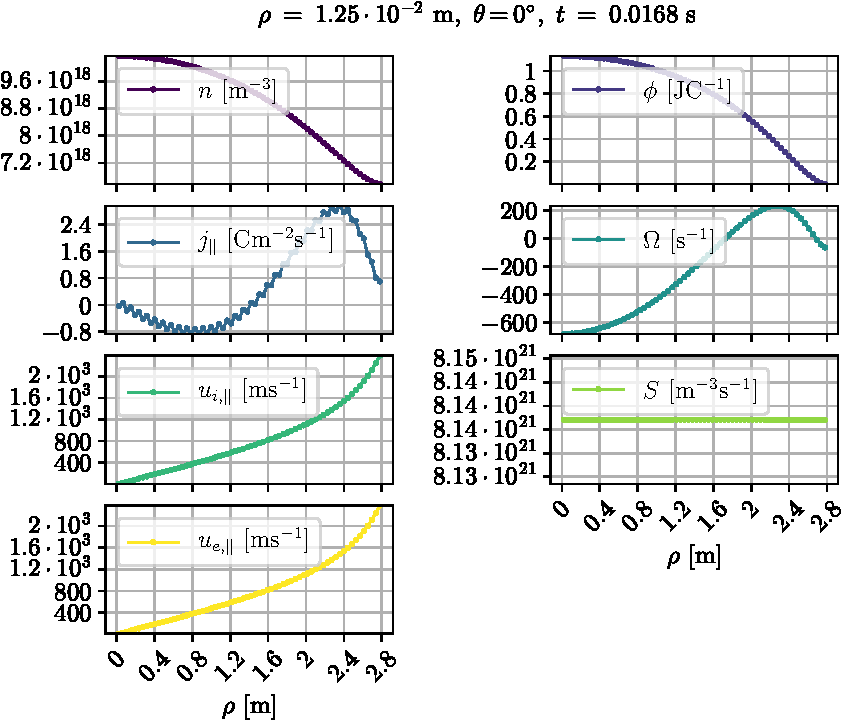
\includegraphics[width=1.0\textwidth]{fig/results/1DProfiles/B010Par}
        \caption{Parallel profiles in steady state}
        \label{fig:parProfs}
    \end{subfigure}%
    \\
    \begin{subfigure}[h]{1.00\textwidth}
        \centering
        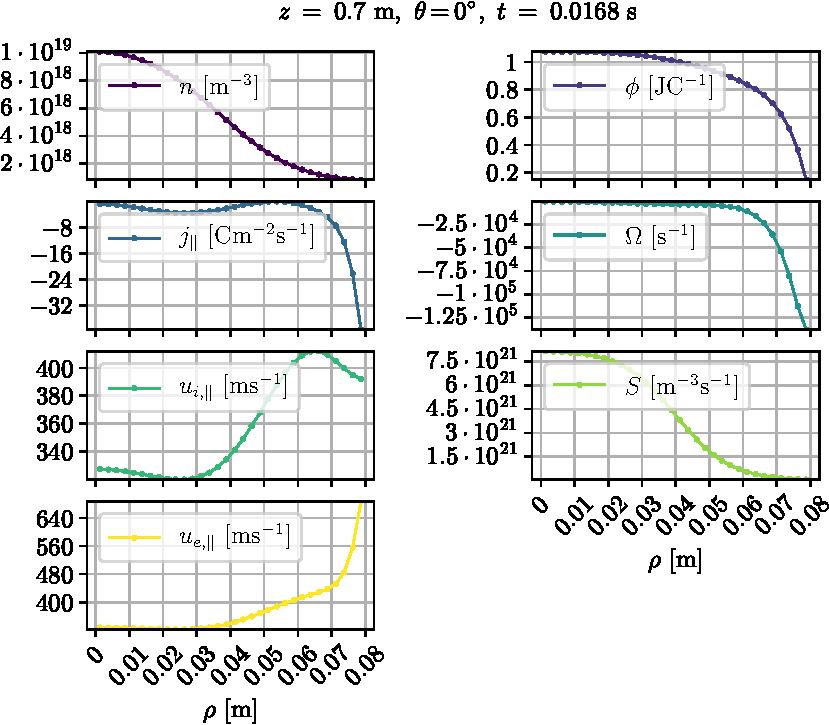
\includegraphics[width=1.0\textwidth]{fig/results/1DProfiles/B010Rad}
        \caption{Radial profiles in steady state}
        \label{fig:radProfs}
    \end{subfigure}
\end{figure}
%
Linear phase, see growing and rotation.
Doesn't start by itself, but is seeded with a Gaussian noise with a level of on vortD
% FIXME; Could add arrow indicating direction of rotation
%
\begin{figure}[htbp]
    \centering
    \begin{subfigure}[h]{1.00\textwidth}
        \centering
        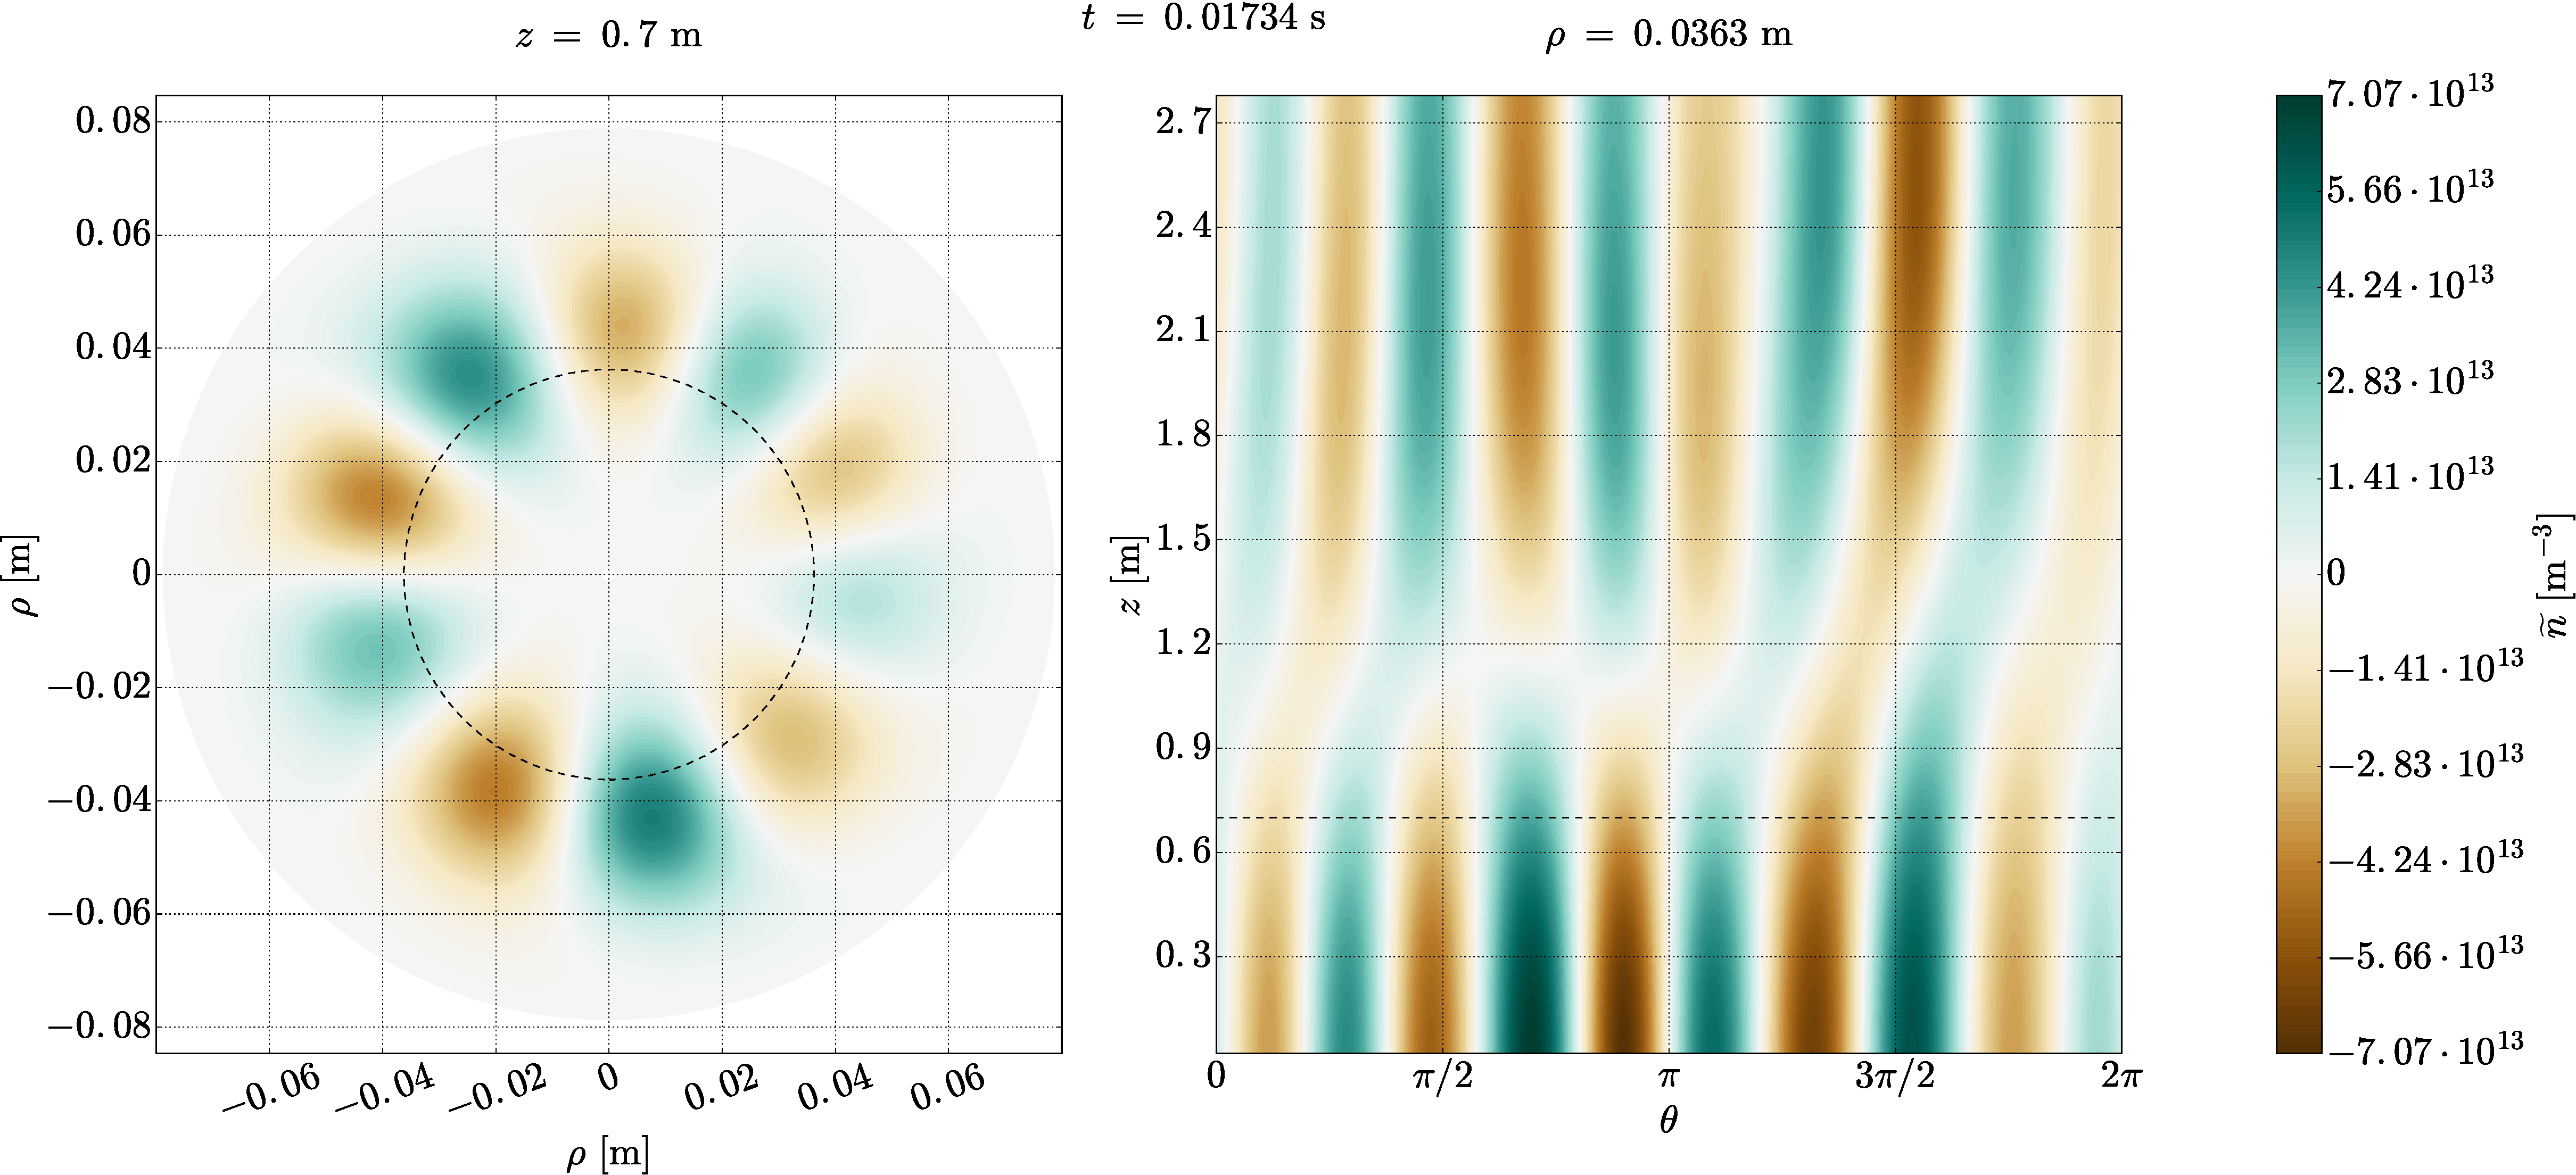
\includegraphics[width=1.0\textwidth]{fig/results/rotModes/n-perpPol-2D-fluct-0}
        \label{fig:rot1}
    \end{subfigure}%
    \\
    \begin{subfigure}[h]{1.00\textwidth}
        \centering
        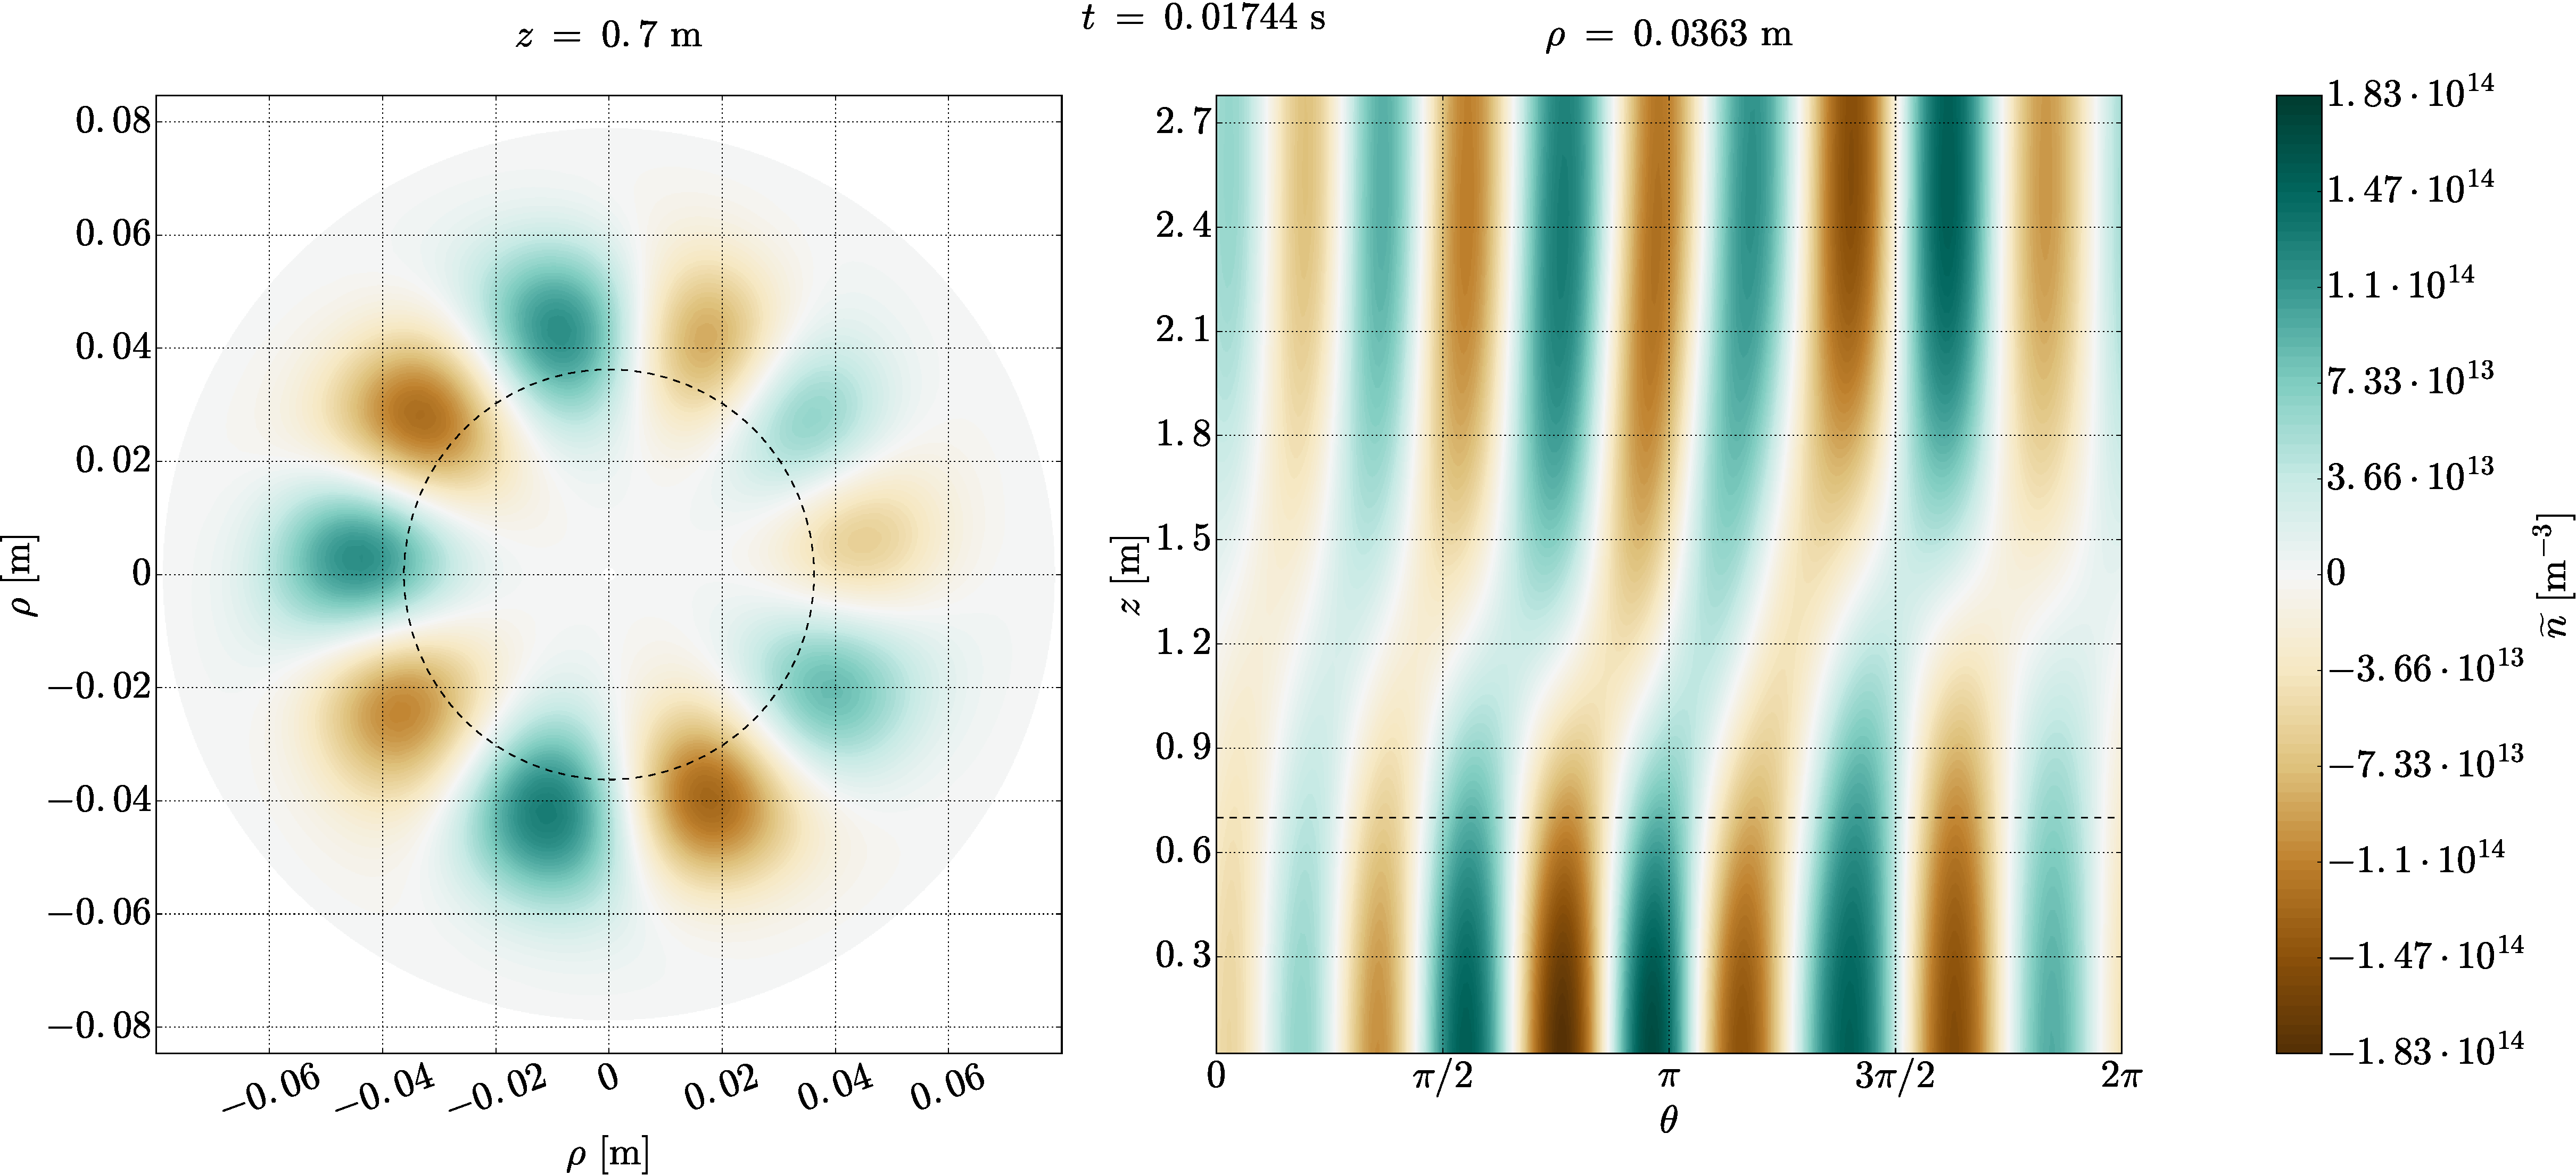
\includegraphics[width=1.0\textwidth]{fig/results/rotModes/n-perpPol-2D-fluct-1}
        \label{fig:rot2}
    \end{subfigure}
    \\
    \begin{subfigure}[h]{1.00\textwidth}
        \centering
        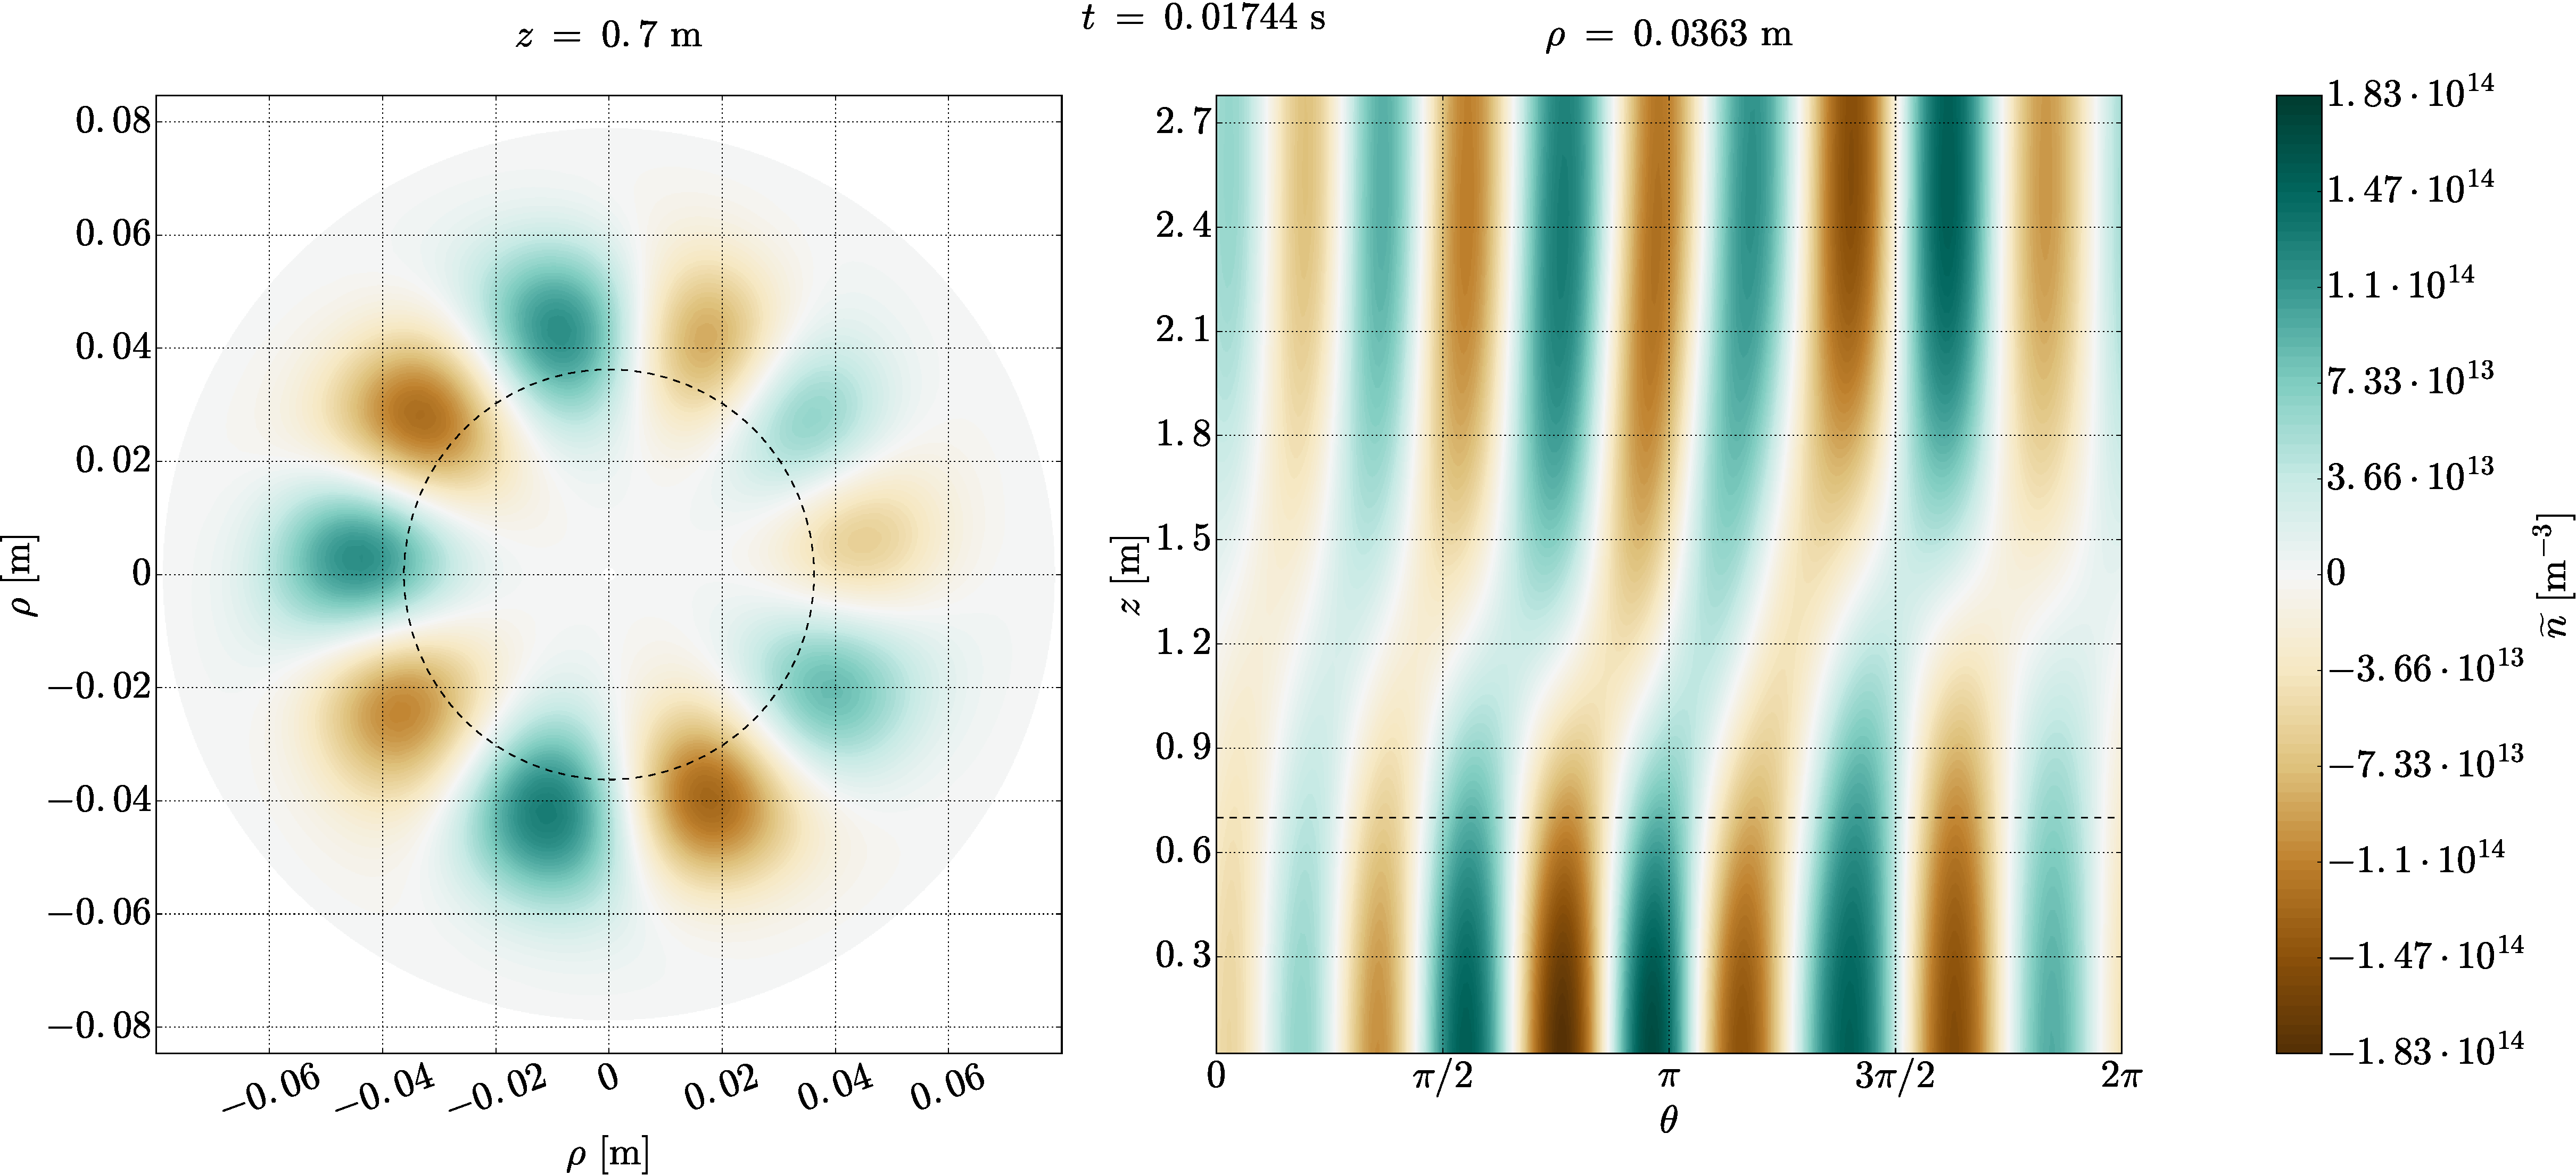
\includegraphics[width=1.0\textwidth]{fig/results/rotModes/n-perpPol-2D-fluct-2}
        \label{fig:rot3}
    \end{subfigure}
    \caption{Rotation of modes}
\end{figure}
%
Dominating mode is dependent on $B$, also, parallel mode moves
%
\begin{figure}[htbp]
    \centering
    \begin{subfigure}[h]{1.00\textwidth}
        \centering
        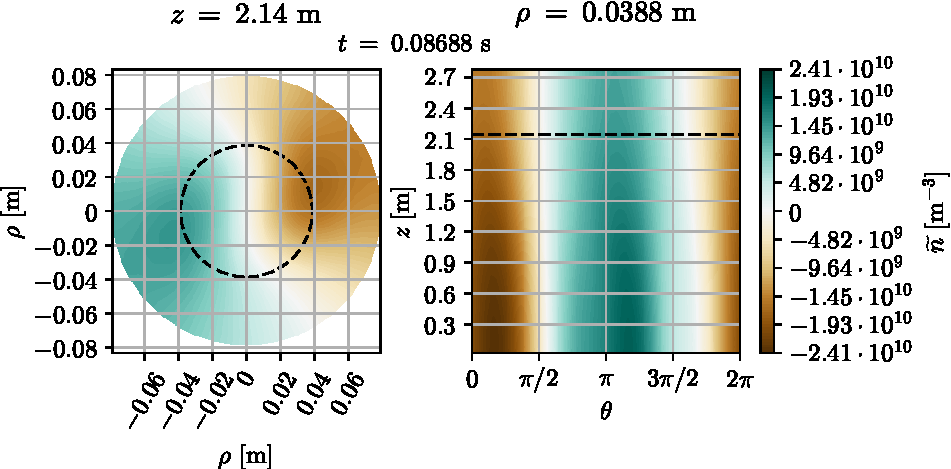
\includegraphics[width=1.0\textwidth]{fig/results/modesDiffScanVals/B002}
        \caption{$B=0.02 \T$}
        \label{fig:B002}
    \end{subfigure}%
    \\
    \begin{subfigure}[h]{1.00\textwidth}
        \centering
        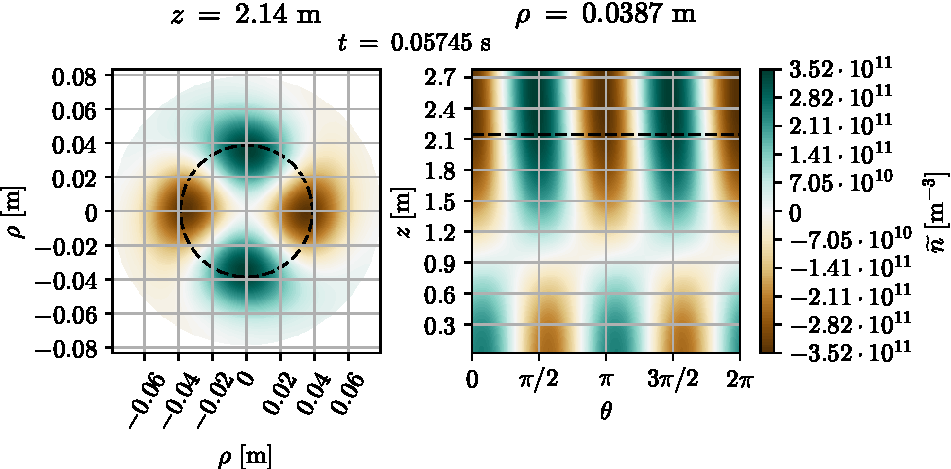
\includegraphics[width=1.0\textwidth]{fig/results/modesDiffScanVals/B004}
        \caption{$B=0.04 \T$}
        \label{fig:B004}
    \end{subfigure}
    \\
    \begin{subfigure}[h]{1.00\textwidth}
        \centering
        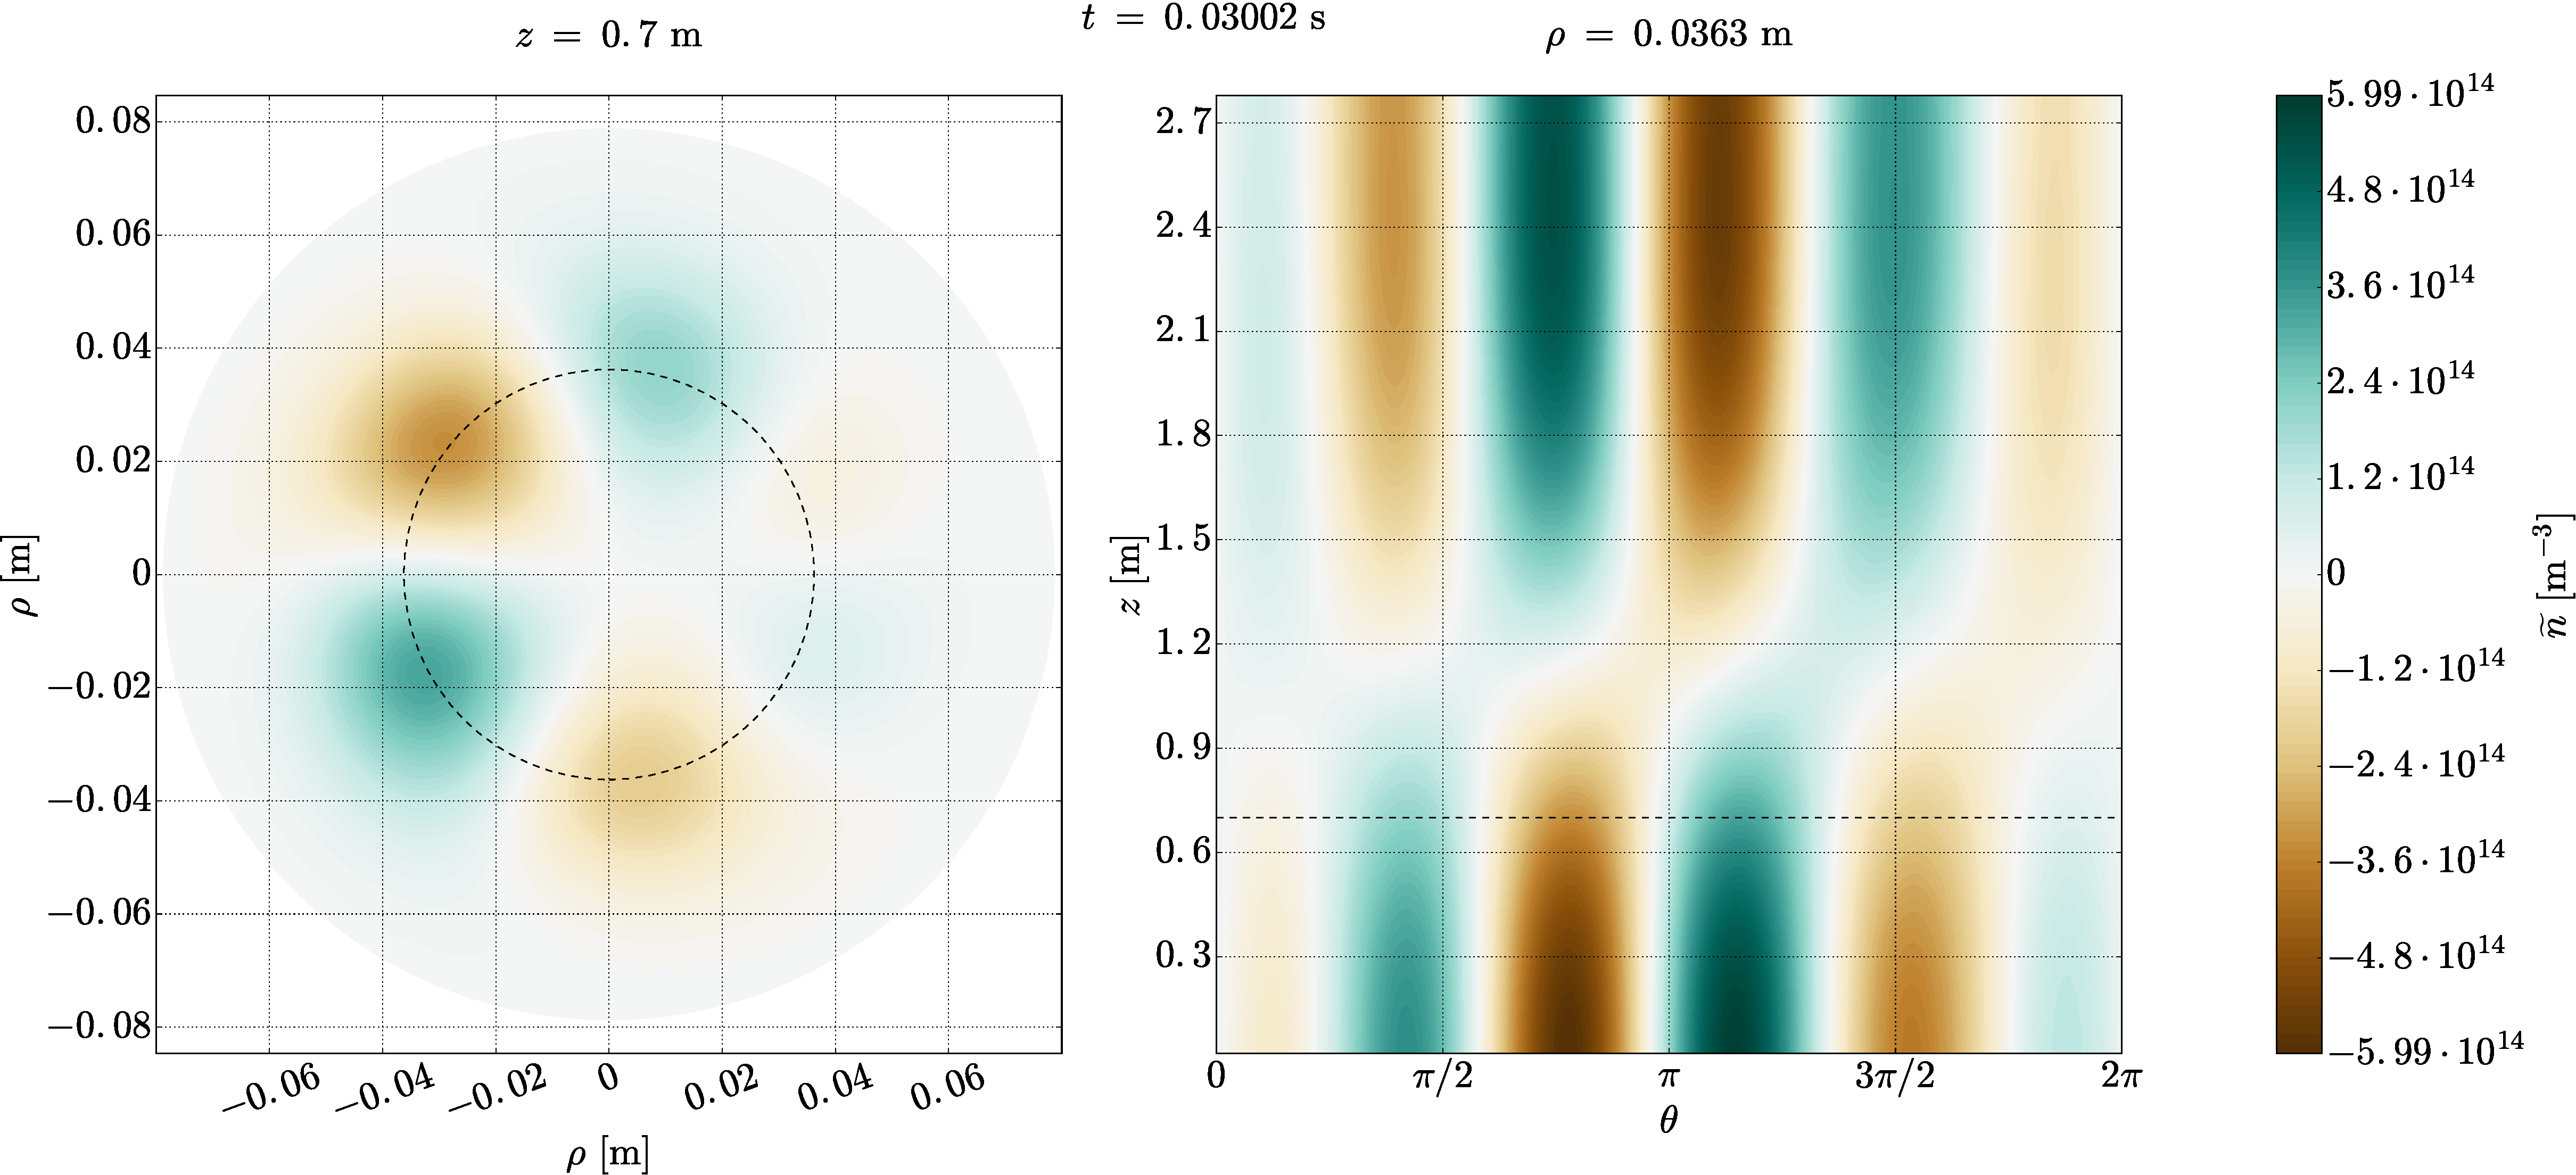
\includegraphics[width=1.0\textwidth]{fig/results/modesDiffScanVals/B006}
        \caption{$B=0.06 \T$}
        \label{fig:B006}
    \end{subfigure}
    \caption{Dominant mode depends on $B$}
\end{figure}
%
A more quantitative way to look at the linear phase is to plot the fourier modes at the position of the most unstable growth.
From theory, this coincides with the position of largest gradient.
As the abscissa is logarithmic, exponential grow will appear as straigth lines
%
\begin{figure}[htbp]
    \centering
    \begin{subfigure}[h]{1.00\textwidth}
        \centering
        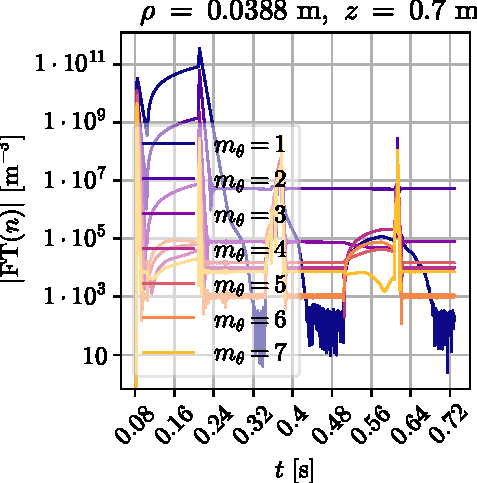
\includegraphics[width=1.0\textwidth]{fig/results/fourierModes/stable}
        \label{fig:fourierStable}
        \caption{For $B=0.02\T$ the system is stable against perturbation}
    \end{subfigure}%
    \\
    \begin{subfigure}[h]{1.00\textwidth}
        \centering
        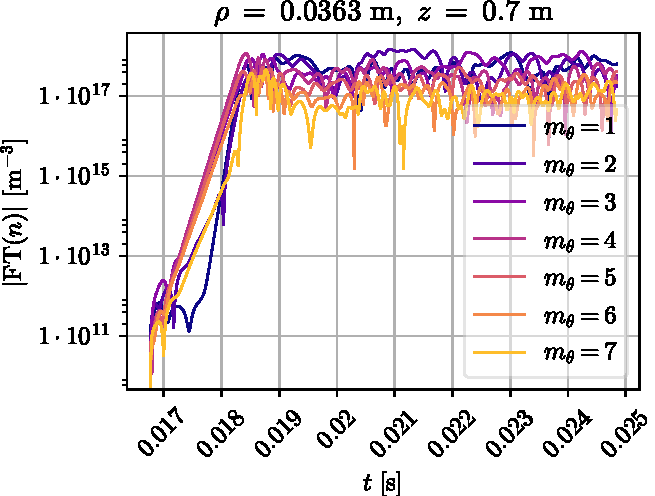
\includegraphics[width=1.0\textwidth]{fig/results/fourierModes/unstable}
        \label{fig:fourierUnstable}
        \caption{Growth rate leading to saturated turbulence for $B=0.1\T$}
    \end{subfigure}
    \caption{Time trace of the Fourier modes.}
\end{figure}
%
Can be summarized in growth rates plot
Assuming perturbation on the from $A\exp\L(i[k_\theta \theta - \L(i\Im[\om] + \Re[\om]\R) t]\R)$, where one can assure oneself that positive $\Im(\om)$ causes exponential growth, and a positive $\Re(\om)$ causes a counter-clockwise rotation of the perturbation if $\theta$ grows in the counter-clockwise direction, as the inverse wavelength $k_\theta$ stays constant.
%
\begin{figure}[htbp]
    \centering
    \begin{subfigure}[h]{1.00\textwidth}
        \centering
        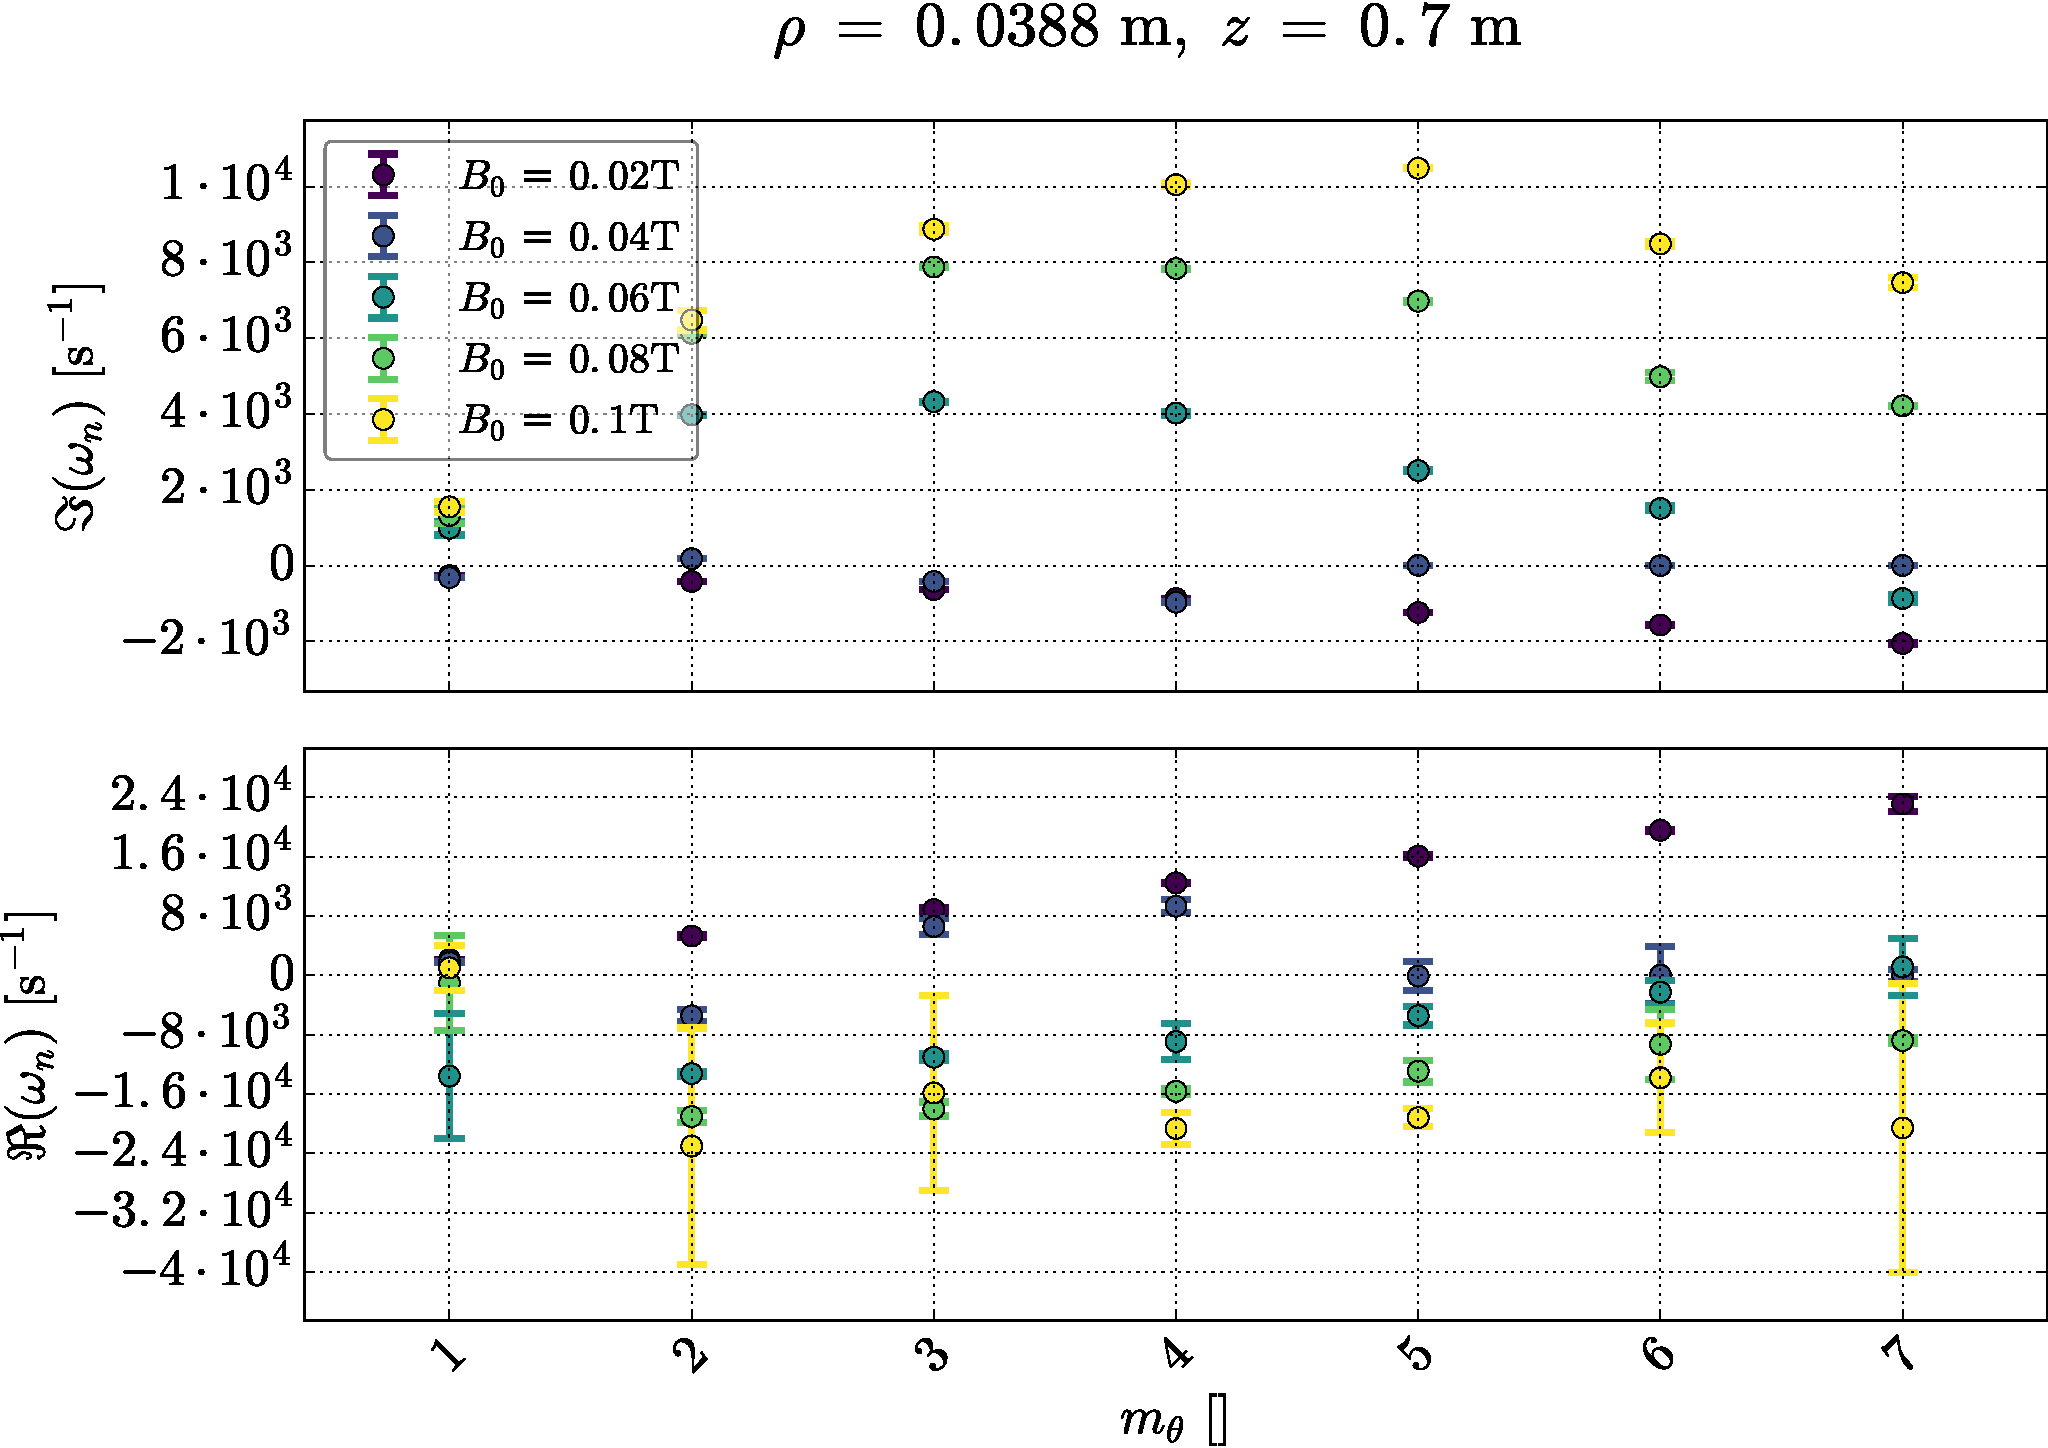
\includegraphics[width=1.0\textwidth]{fig/results/growthRates/growthRatesB0}
        \label{fig:grB}
    \end{subfigure}%
    \\
    \begin{subfigure}[h]{1.00\textwidth}
        \centering
        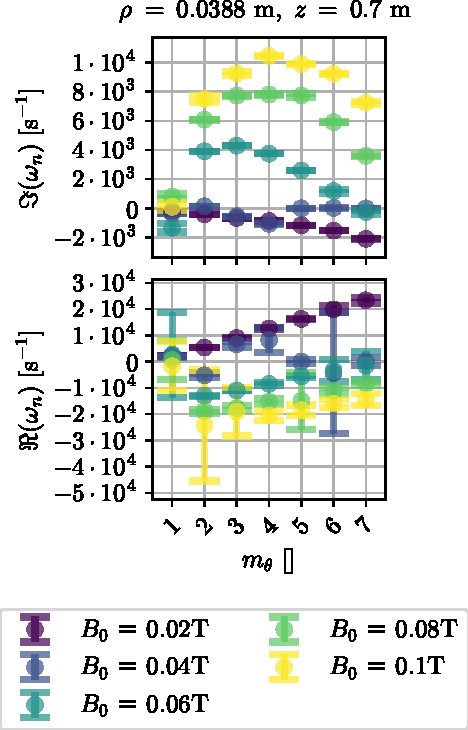
\includegraphics[width=1.0\textwidth]{fig/results/growthRates/growthRatesB0ModeNr}
        \label{fig:grBModeNr}
    \end{subfigure}
    \caption{$B$-dependency on growth rates}
\end{figure}
%
Finally lead to the turbulent state.
On the transition from the linear phase to the turbulent phase a energy overshot is observed.
As a consequence the eddies evolve at a faster phase, before the saturated turbulent state where eddies evolve at a slower rate, and the energy stays closer to the temporal mean (as seen in ...)
It is also important to observe that the fluctations can be big enough to push the plasma off center as observed in ...
%
\begin{figure}[htbp]
    \centering
    \begin{subfigure}[h]{1.00\textwidth}
        \centering
        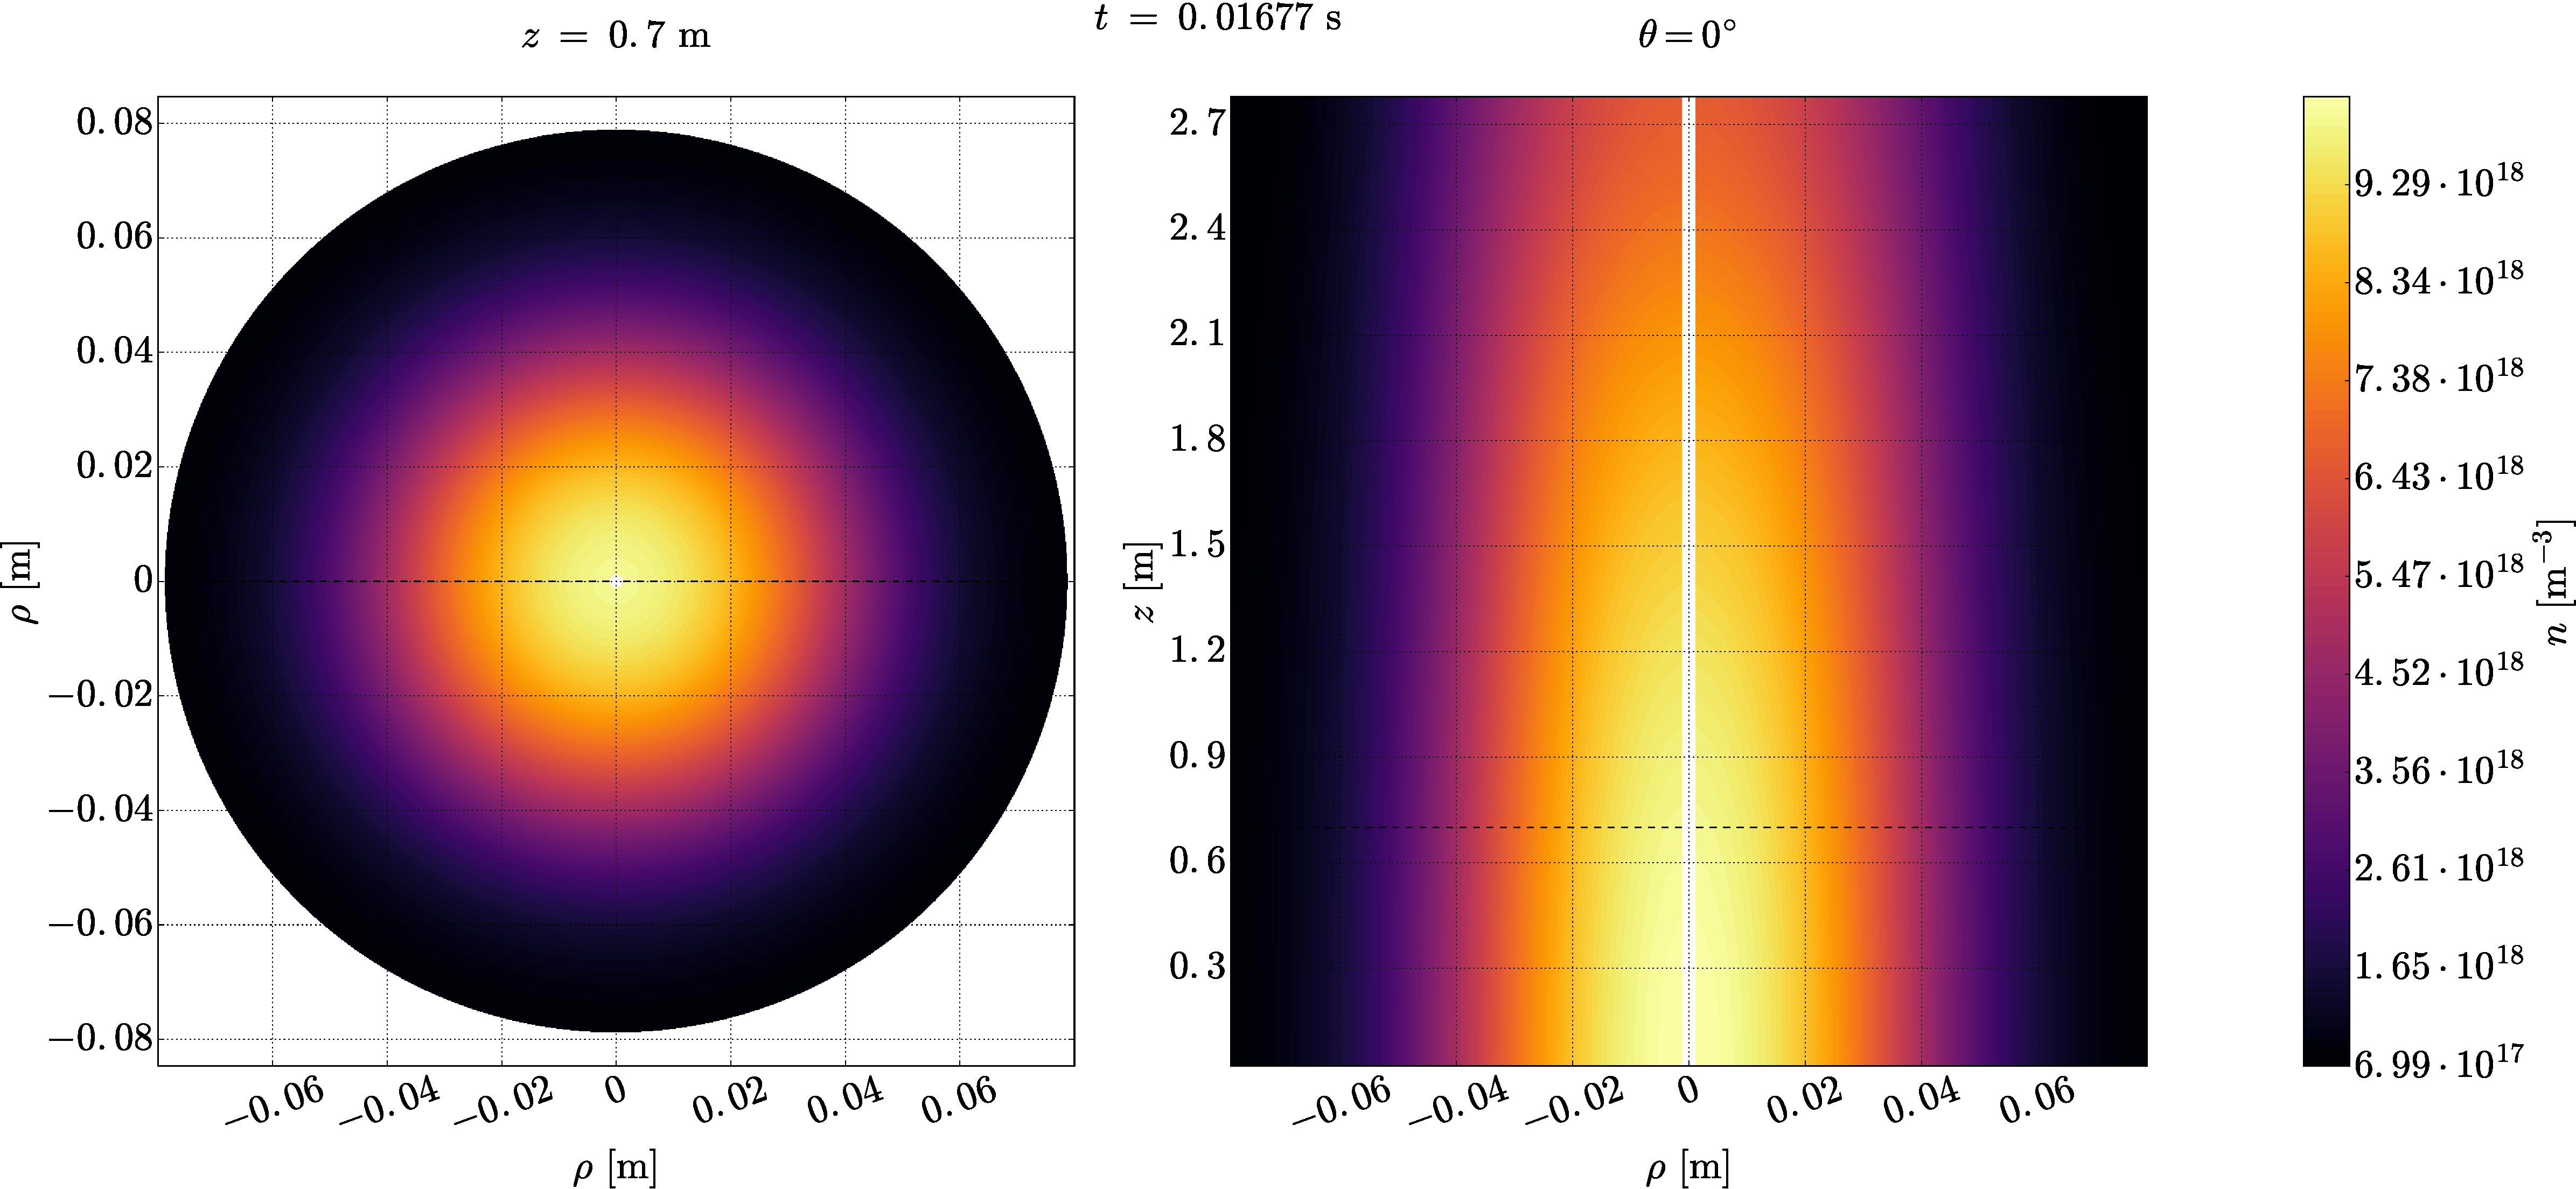
\includegraphics[width=1.0\textwidth]{fig/results/2DTurbulence/steadyStateN}
        \caption{The plasma at the steady state.}
        \label{fig:2Dsteady}
    \end{subfigure}%
    \\
    \begin{subfigure}[h]{1.00\textwidth}
        \centering
        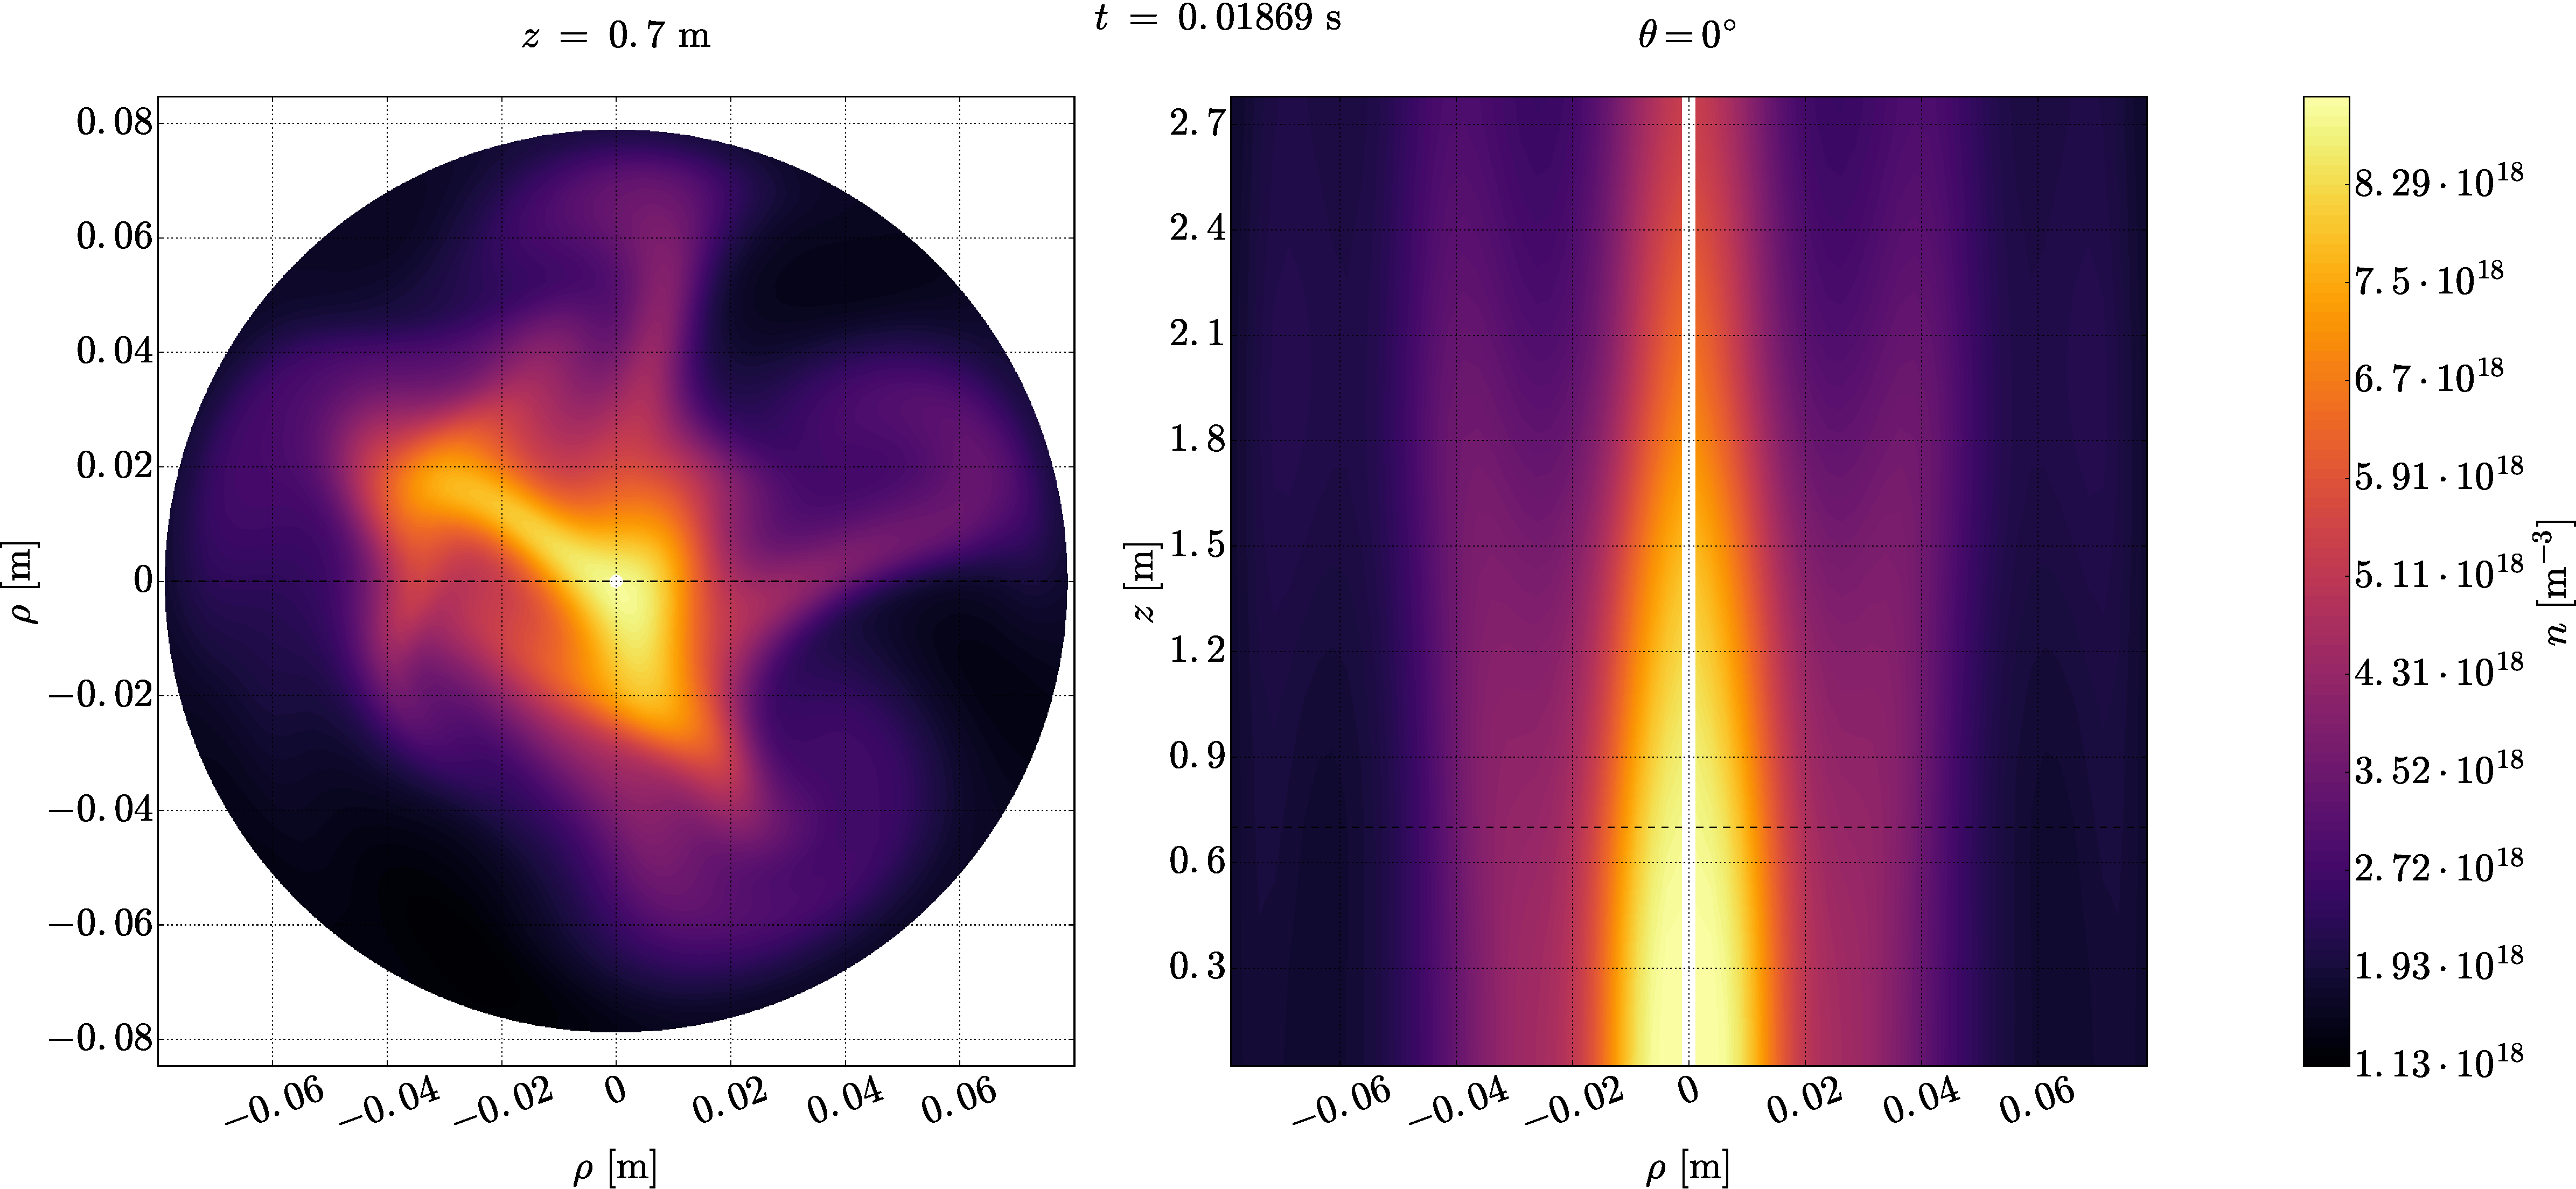
\includegraphics[width=1.0\textwidth]{fig/results/2DTurbulence/violentBurst}
        \caption{A violent burst is observed at the energy overshoot.}
        \label{fig:violentBurst}
    \end{subfigure}
    \\
    \begin{subfigure}[h]{1.00\textwidth}
        \centering
        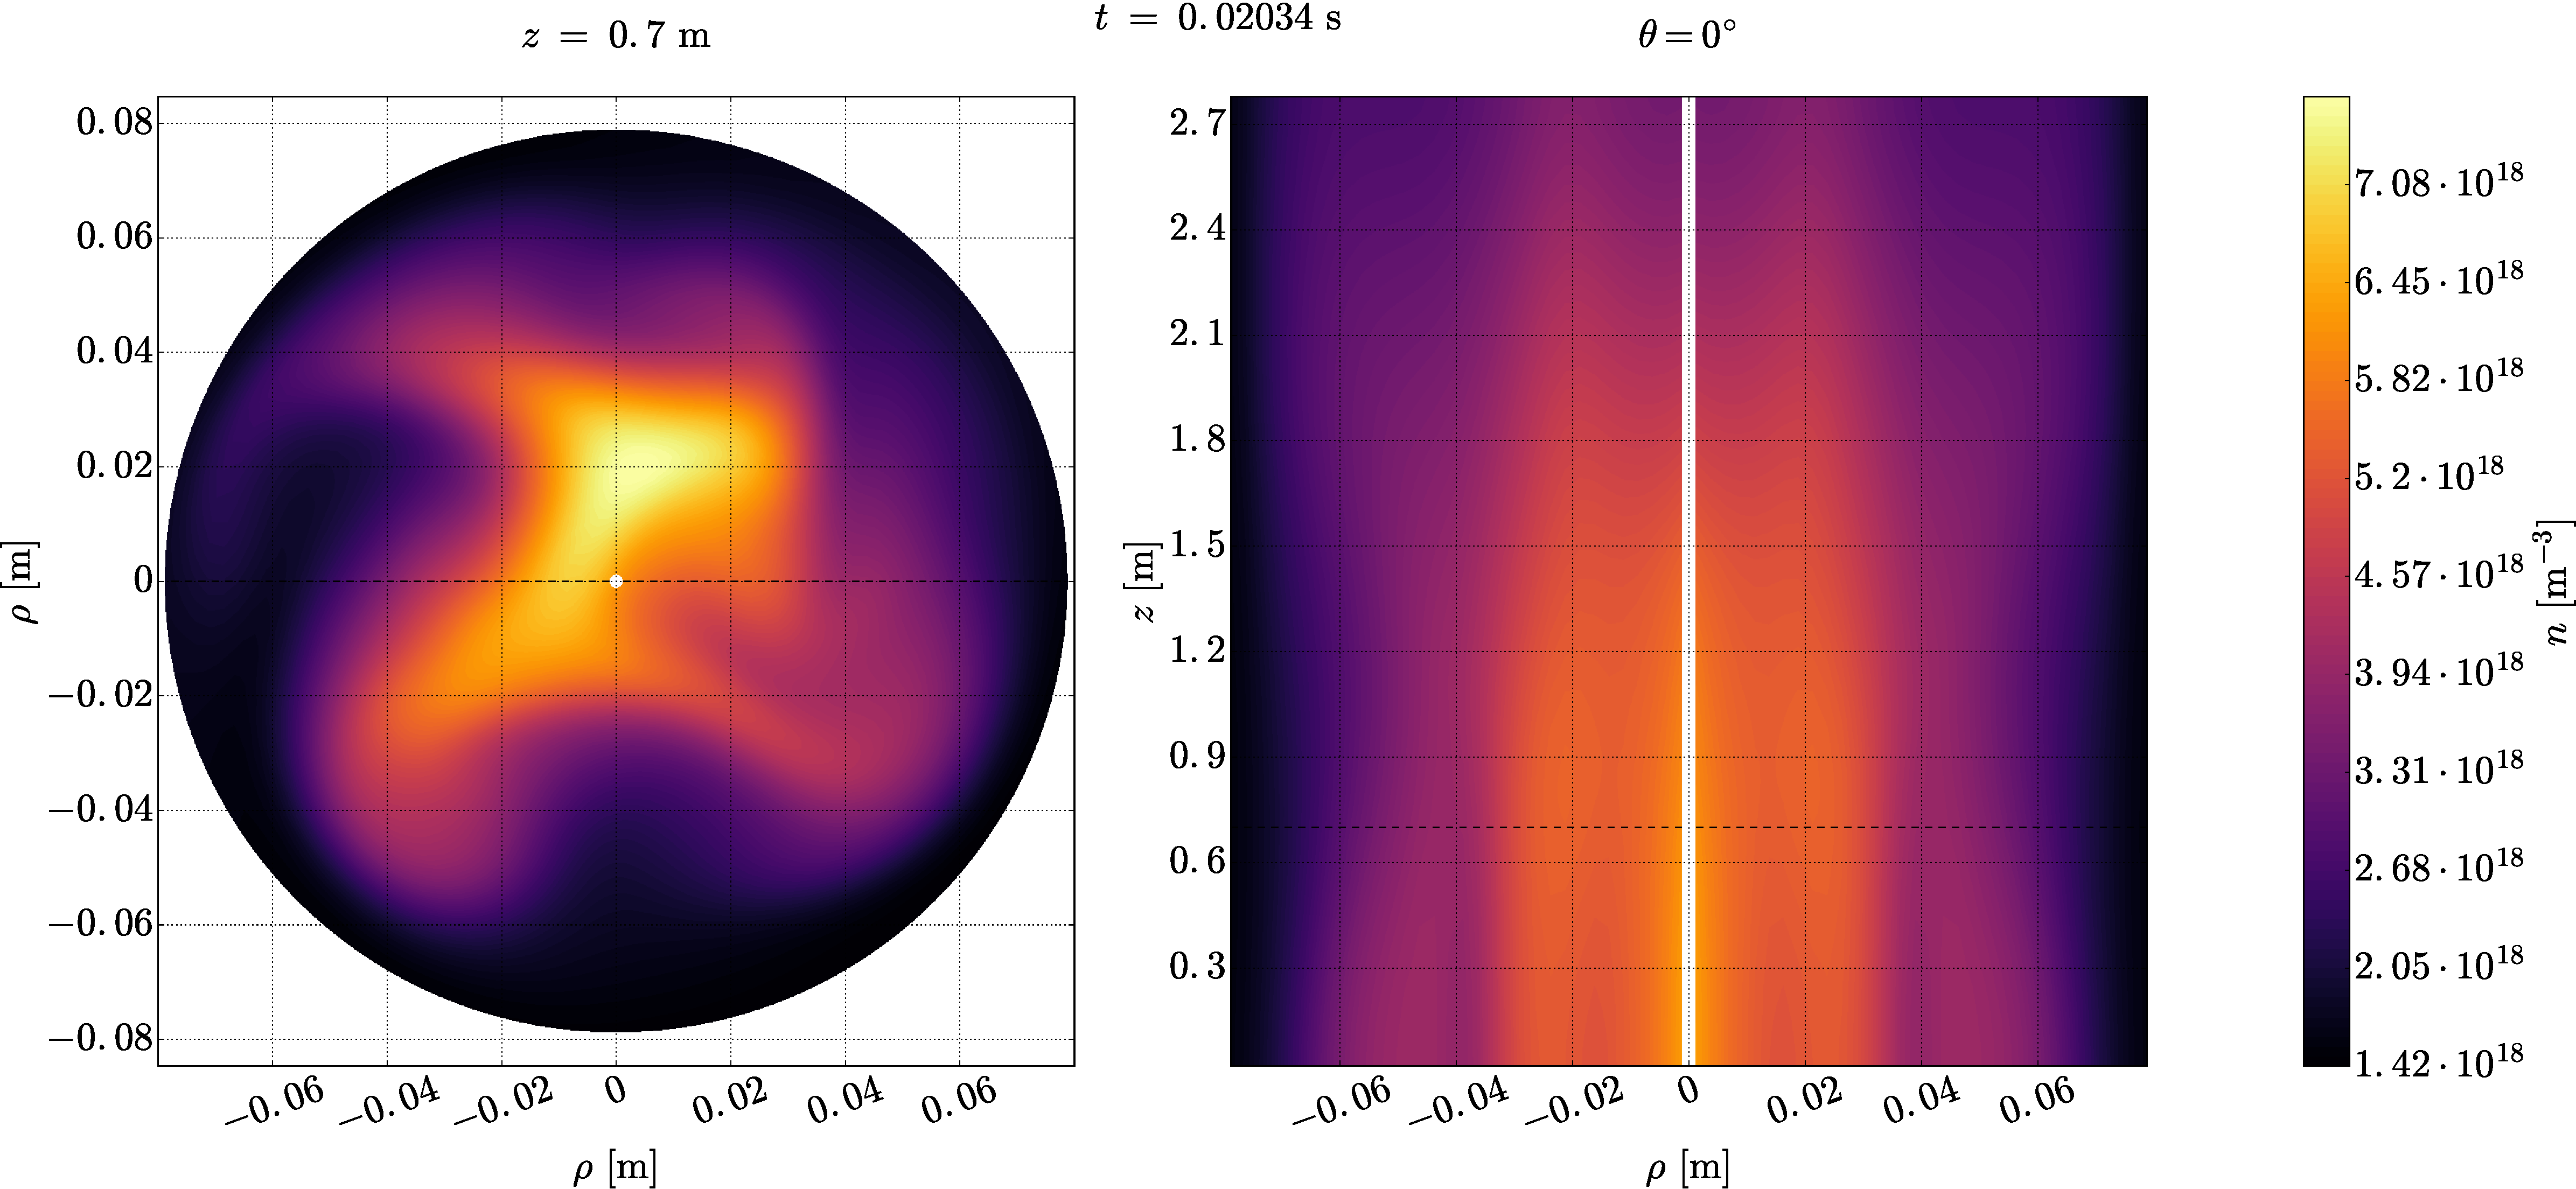
\includegraphics[width=1.0\textwidth]{fig/results/2DTurbulence/offCenter}
        \caption{$B=0.06 \text{T}$}
        \label{fig:offcenter}
    \end{subfigure}
    \caption{Turbulent eddies are observed in the saturated turbulence state.
    Here shown for $B=0.1\T$}
\end{figure}
%
The fluctuations are no longer in an ordered pattern as they were in the linear phase, as shown in
%
\begin{figure}[htb]
    \centering
    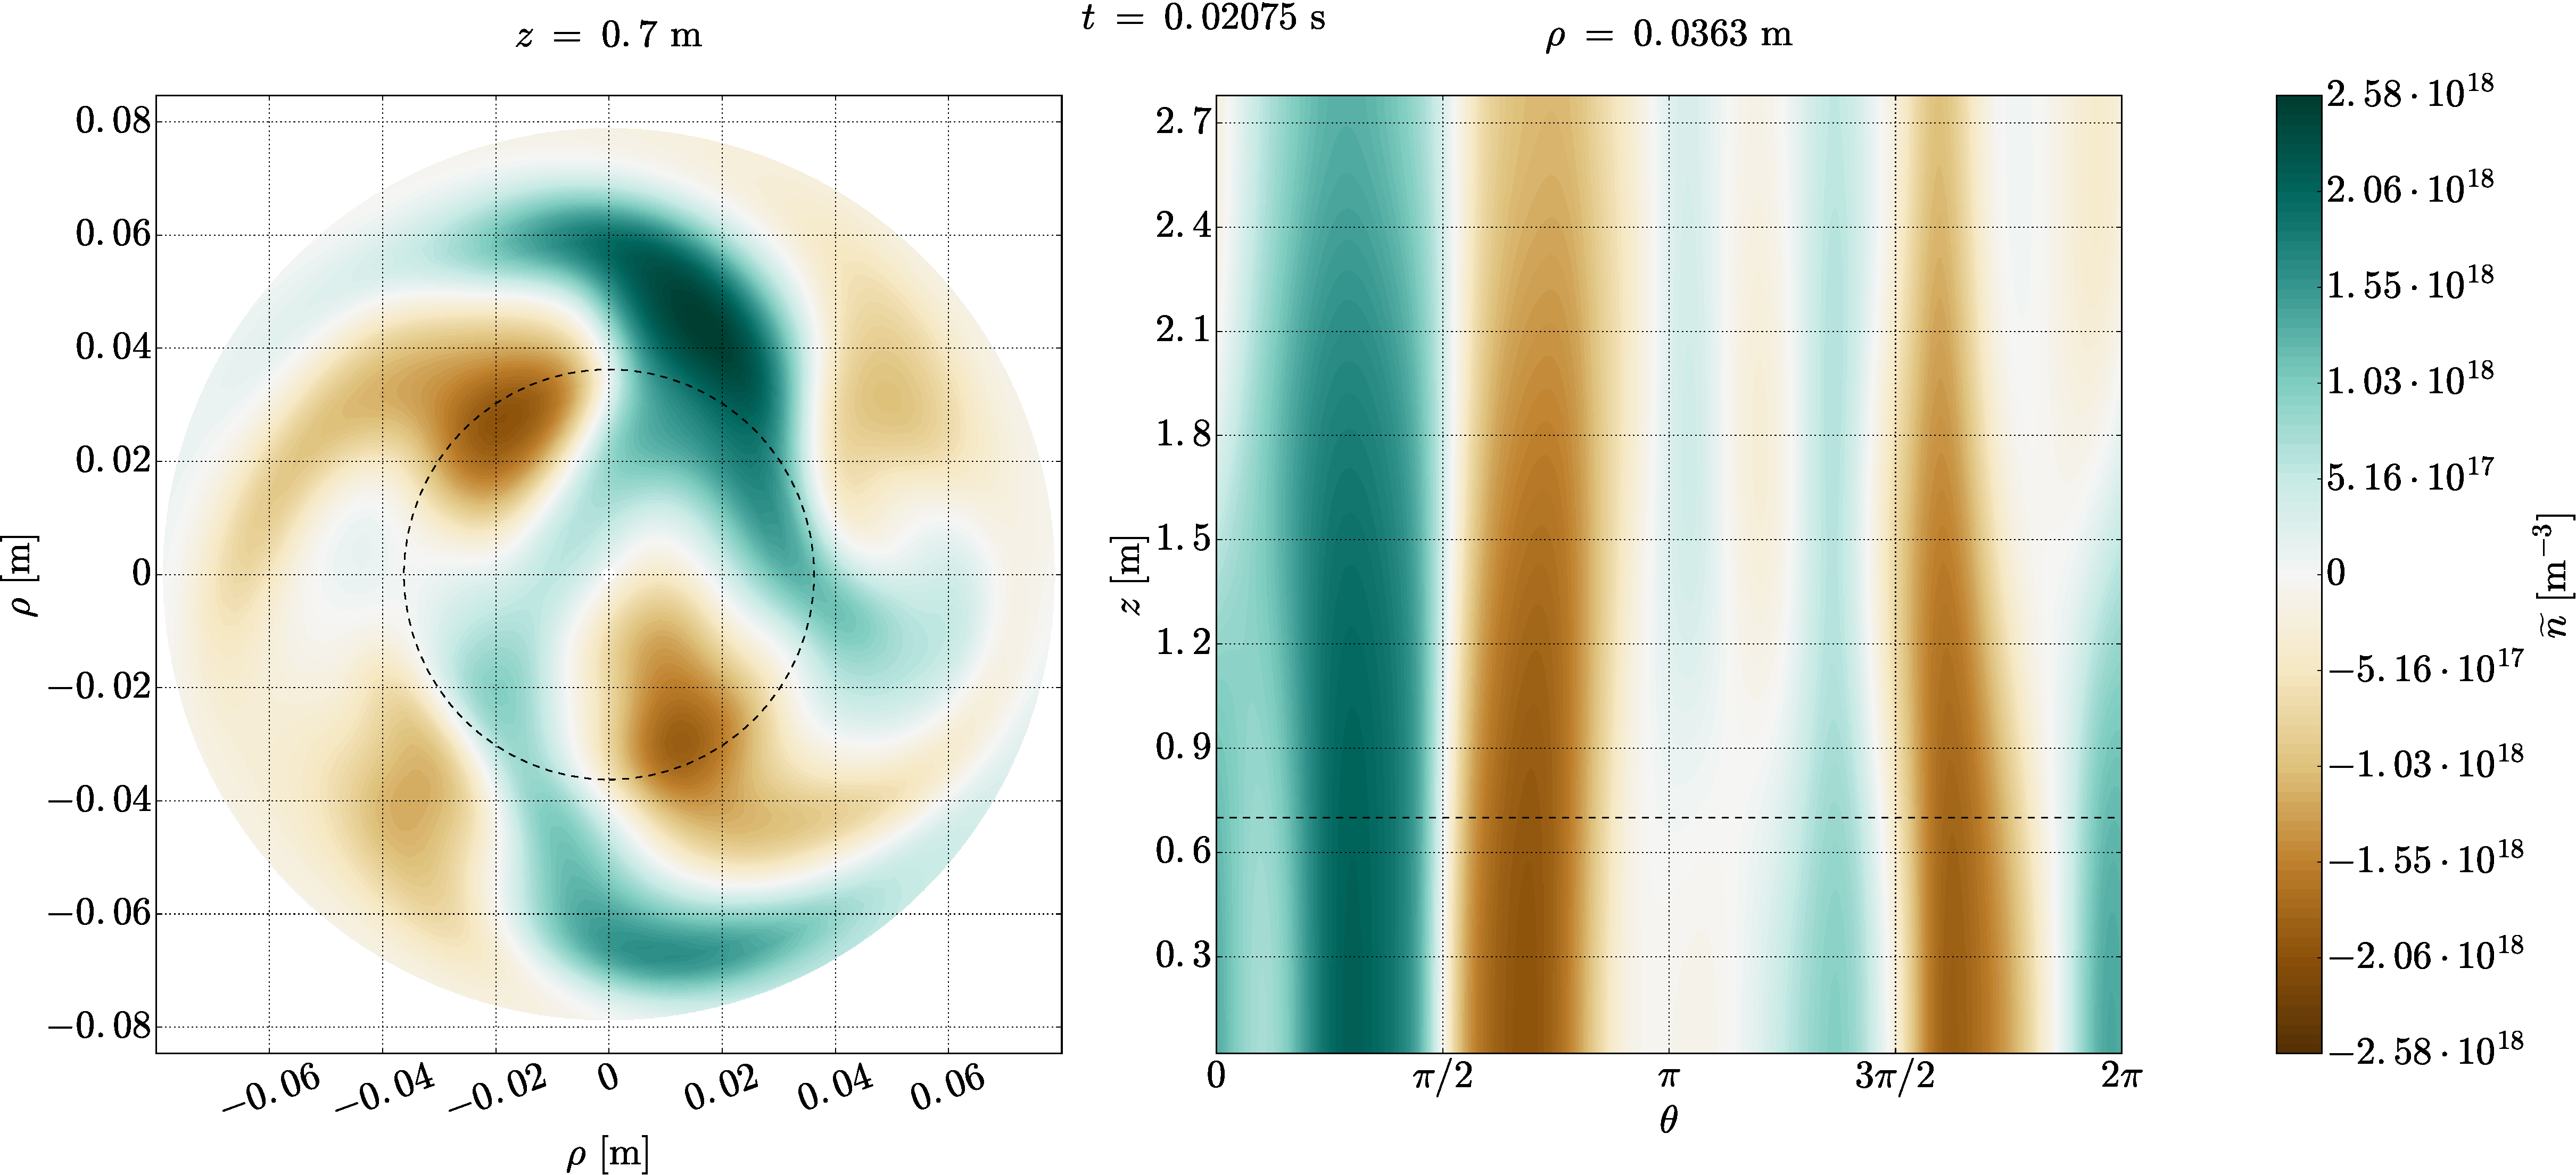
\includegraphics[width=1.0\textwidth]{fig/results/2DTurbulence/fluct}
    \caption{\textit{Fluctations in the turbulent state for $B=0.1\T$}}
    \label{fig:divDDZ}
\end{figure}
